\chapter{Как быстро идут химические реакции}

\section{Что такое скорость реакции}

В предыдущей главе мы разобрались, при каких условиях химическая реакция является самопроизвольной, а при каких будет протекать обратный процесс. При этом термодинамика совершенно не отвечает на вопрос \emph{как быстро будет происходить реакция}. Из своего жизненного опыта вы знаете, что некоторые реакции происходят практически мгновенно (например, взрыв), иногда в течение нескольких минут (горение древесины), иногда в течение нескольких лет (ржавление железа), а иногда и целых эпох (выветривание горных пород).

Однако для точной науки слов <<быстро>> и <<медленно>> недостаточно, нужны числовые значения. Вы уже встречали знак $\tau$ над стрелкой в уравнении реакции (табл.~\ref{tab:designation_of_reaction_conditions}), который показывает, что реакции требуется время. Теперь мы научимся определять, сколько именно.

В этой главе мы постараемся ответить на три главных вопроса:

\begin{itemize}
    \item как количественно описать, насколько быстро идёт реакция;
    \item от чего зависит скорость реакции и как ею управлять;
    \item может ли скорость реакции рассказать о её механизме.
\end{itemize}

Раздел химии, который изучает скорости химических реакций и то, \emph{каким путём} они протекают, называется \term{химической кинетикой}{chemical_kinetics}{химическая кинетика} (от греч. \grk{k'inhsis} (\textit{k\'{\i}n\={e}sis})~--- движение).

\subsection*{О скорости}

\emph{Скорость}~--- это изменение, происходящее за определённый промежуток времени. Например, скорость автомобиля принято определять в количестве километров, которые он проезжает за один час. Банковскую ставку (это тоже скорость) определяют как количество процентов от суммы вашего вклада, на которые увеличится ваша сумма за один год. Таким образом, в общем виде

\begin{equation}
    \label{eq:definition_of_speed}
    \text{Скорость} = \frac{\text{Изменение}}{\text{Промежуток времени}}.
\end{equation}

Когда мы говорим о скорости химической реакции, то логично использовать изменение количеств (концентраций) веществ в ходе реакции. При этом концентрация исходных веществ будет уменьшаться, а продуктов~--- расти.

В зависимости от того, какую химическую систему мы рассматриваем, числитель выражения \eqref{eq:definition_of_speed} можно выразить в любых величинах, отражающих изменение количеств веществ в реакции, например, в виде изменения \emph{концентрации вещества} (в случае растворов), \emph{парциального давления} (в случае газов это эквивалентно концентрации), \emph{единиц длины} (при рассмотрении глубины коррозии), просто в молях и т.~п.

\subsection*{Кинетическая кривая}

Для изучения скорости реакции наиболее удобно представить величины, связанные с изменением количеств веществ, в виде графика зависимости от времени. Такой график называют \term{кинетической кривой}{kinetic_curve}{кинетическая кривая}. Для построения такого графика сначала строят таблицу, измеряя концентрации веществ через определённые промежутки времени, а затем наносят эти точки на график. Например, в таблице~\ref{tab:ethanol_in_blood} представлены концентрации этанола в крови человека после внутривенного введения, а на рис.~\ref{fig:ethanol_in_blood}~--- кинетическая кривая, построенная на её основе.

\begin{table}[htbp]
    \small
    \caption{Концентрация этанола в крови человека после внутривенного введения.}
    \label{tab:ethanol_in_blood}
    \begin{tabularx}{\textwidth}{
        >{\hsize=1\hsize}Z
        >{\hsize=1\hsize}Z
        >{\hsize=1\hsize}Z
        }
        \hline
        \rowcolor{table_header}
        $t$, \unit{\ruCh} & $c(\ce{C2H5OH})$, \unit{\ruMmole\per\ruL} & $c(\ce{C2H5OH})$, \unit{\ruG\per\ruL} \\
        \hline
        0 & \num{35,0} & \num{1,61} \\
        1 & \num{31,7} & \num{1,46} \\
        2 & \num{28,4} & \num{1,31} \\
        3 & \num{25,1} & \num{1,16} \\
        4 & \num{21,8} & \num{1,00} \\
        5 & \num{18,5} & \num{0,85} \\
        6 & \num{15,2} & \num{0,70} \\
        7 & \num{11,9} & \num{0,55} \\
        8 & \num{8,6} & \num{0,40} \\
        9 & \num{5,3} & \num{0,24} \\
        \hline
    \end{tabularx}
\end{table}

\begin{figure}[htbp]
    \centering
    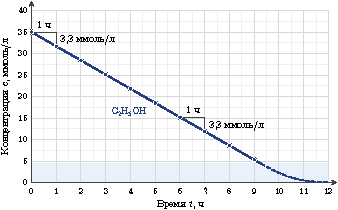
\includegraphics[width=12cm]{figs/what_is_reaction_rate/ethanol_zero_order.pdf}
    \caption{График на основании таблицы~\ref{tab:ethanol_in_blood}.}
    \label{fig:ethanol_in_blood}
\end{figure}

Как мы видим, концентрация этанола в крови изменяется линейно, равномерно убывая через равные промежутки времени, исключая период, когда этанол почти полностью метаболизирован.

Однако кинетическая кривая не всегда является линейной. Давайте рассмотрим изученную в 1930~году Эйрингом и Даниэлсом реакцию разложения при \qty{45}{\degreeCelsius} оксида азота (V)\footnote{H. Eyring, F. Daniels. J. Am. Chem. Soc. 52, 1472 (1930), табл. II, опыт 2.}, растворённого в \ce{CCl4}:

\reaction[ce:n2o5_decomposition]{2N2O5 -> 2N2O4 + O2 (^) {.}}

Тетраоксид диазота \ce{N2O4} остаётся в растворе, а кислород выделяется из него в виде газа\footnote{Сначала образуется диоксид азота в ходе реакции \ce{2N2O5 -> 4NO2 + O2}. Затем, как вы помните из задачи~\ref{prob:gibbs_energy2}, молекулы \ce{NO2} объединяются в \ce{N2O4}, поэтому уравнение записано сразу с \ce{N2O4}. Тем не менее раствор всё равно будет выглядеть бурым из-за небольшого количества \ce{NO2}.}. Концентрацию \ce{N2O5} определяли в разные моменты времени, результаты показаны в табл.~\ref{tab:n2o5_decomposition}\footnote{В статье для каждого момента времени указан объём кислорода, который \emph{ещё выделится} до конца реакции. Этот объём пропорционален количеству оставшегося \ce{N2O5}, по нему вычисляется концентрация \ce{N2O5}, а концентрации \ce{N2O4}~--- по уравнению~\eqref{ce:n2o5_decomposition}.}.

\begin{table}[htbp]
    \small
    \caption{Разложение \ce{N2O5} в растворе в \ce{CCl4} при \qty{45}{\degreeCelsius}.}
    \label{tab:n2o5_decomposition}
    \begin{tabularx}{\textwidth}{
        >{\hsize=1\hsize}Z
        >{\hsize=1\hsize}Z
        >{\hsize=1\hsize}Z
        }
        \hline
        \rowcolor{table_header}
        $t$, с & $c(\ce{N2O5})$, \unit{\ruMole\per\ruL} & $c(\ce{N2O4})$, \unit{\ruMole\per\ruL} \\
        \hline
        0 & \num{2,33} & 0 \\
        \num{184} & \num{2,07} & \num{0,26} \\
        \num{319} & \num{1,91} & \num{0,42} \\
        \num{526} & \num{1,68} & \num{0,65} \\
        \num{867} & \num{1,35} & \num{0,98} \\
        \num{1198} & \num{1,11} & \num{1,22} \\
        \num{1877} & \num{0,72} & \num{1,61} \\
        \hline
    \end{tabularx}
\end{table}

Построим кинетические кривые для реагента и основного продукта (рис.~\ref{fig:kinetic_curves}). Поскольку реагент расходуется в реакции, то его кривая идёт вниз, а концентрация продукта растёт (кривая идёт вверх), причём кривые являются взаимным отражением друг друга, потому что по уравнению~\eqref{ce:n2o5_decomposition} на каждую разложившуюся молекулу \ce{N2O5} образуется одна молекула \ce{N2O4}.

\begin{figure}[htbp]
    \centering
    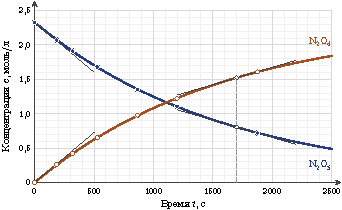
\includegraphics[width=12cm]{figs/what_is_reaction_rate/kinetic_curves.pdf}
    \caption{Кинетические кривые разложения \ce{N2O5} в растворе в \ce{CCl4} при \qty{45}{\degreeCelsius}. Закрашенные точки~--- концентрации \ce{N2O5}, полученные в результате эксперимента, незакрашенные~--- концентрации \ce{N2O4}, вычисленные по уравнению реакции. Отрезками показаны касательные к обеим кривым в начальный момент времени и в момент $t = \qty{1700}{\ruS}$.}
    \label{fig:kinetic_curves}
\end{figure}

Обратите внимание на форму кинетических кривых. В отличие от случая разложения этанола в крови, они не являются линейными. В начальный момент времени концентрации меняются быстро, но чем дольше протекает реакция, тем медленнее это происходит. За первые \qty{526}{\ruS} концентрация \ce{N2O5} упала на \qty{0,65}{\ruMole\per\ruL}, а за \qty{679}{\ruS} между 1198-й и 1877-й секундами~--- всего на \qty{0,39}{\ruMole\per\ruL}, хотя этот промежуток даже длиннее. Другими словами, реакция постепенно замедляется. Это означает, что в данном случае не существует единой скорости на всём времени протекания реакции и можно говорить о скорости только применительно к определённому промежутку или моменту времени.

Почему скорость в данном случае не остаётся постоянной? По мере протекания реакции молекулы \ce{N2O5} расходуются, превращаясь в продукты, и их остаётся всё меньше в одном и том же объёме раствора. При этом в любой момент времени (и в начале, и в конце реакции) вероятность превращения за единицу времени для каждой из оставшихся молекул всегда остаётся той же самой. В данном случае за любые \qty{650}{\ruS} разлагается примерно треть тех молекул \ce{N2O5}, которые были в растворе в начале этого промежутка времени (рис.~\ref{fig:constant_fraction}). В каждом промежутке реагирует треть от всё меньшего числа молекул, поэтому мы видим, как за одно и то же время распадается всё меньше \ce{N2O5}.

\begin{figure}[htbp]
    \centering
    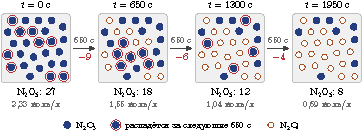
\includegraphics[width=12cm]{figs/what_is_reaction_rate/constant_fraction.pdf}
    \caption{Почему разложение \ce{N2O5} замедляется. Одна и та же порция раствора представлена в моменты \num{0}, \num{650}, \num{1300} и \qty{1950}{\ruS}. 27 молекул соответствуют начальной концентрации \qty{2,33}{\ruMole\per\ruL}. За каждые \qty{650}{\ruS} распадается треть имеющихся молекул \ce{N2O5} (они обведены), но число распадов уменьшается (\num{9}, \num{6} и \num{4}). На месте каждой распавшейся молекулы \ce{N2O5} показана молекула \ce{N2O4}.}
    \label{fig:constant_fraction}
\end{figure}

Почему же, спросите вы, в таком случае скорость распада этанола остаётся одной и той же на протяжении почти всего времени? Дело в том, что этанол в печени окисляется ферментом \emph{алкогольдегидрогеназой}, которого имеется весьма ограниченное количество. Из-за этого скорость зависит просто от того, сколько фермента имеется в организме (каждая молекула фермента оказывается занята процессом, и оставшийся этанол <<ждёт>> своей очереди), а не от концентрации молекул этанола. Когда этанола становится мало, фермент начинает простаивать, и скорость падает~--- это отвечает закрашенной области на рис.~\ref{fig:ethanol_in_blood}.

\subsection*{Средняя скорость}

Скорость реакции на каком-то промежутке времени проще всего описать, разделив изменение концентрации на длительность этого промежутка. В этом случае мы получим \term{среднюю скорость}{average_rate}{средняя скорость} на промежутке времени от $t_1$ до $t_2$. Для реагента A
\begin{equation}
    \label{eq:average_rate}
    \overline{v}(\mathrm{A}) = -\frac{\Delta c(\mathrm{A})}{\Delta t} = -\frac{c_2 - c_1}{t_2 - t_1},
\end{equation}
где $c_1$ и $c_2$~--- его концентрации в моменты $t_1$ и $t_2$. Минус здесь нужен из-за того, что концентрация реагента уменьшается и $\Delta c < 0$ (а скорость принято считать положительной). Для продукта B концентрация растёт, поэтому минус не нужен: $\overline{v}(\mathrm{B}) = \Delta c(\mathrm{B})/\Delta t$.

Скорость, найденную по изменению концентрации одного вещества, называют \term{скоростью по этому веществу}{rate_by_substance}{скорость по веществу}. Для реагента это скорость его \emph{расходования}, для продукта~--- скорость \emph{образования}. Измеряют её в \unit{\ruMole\per\ruL\ruS}.

\begin{example}{}{what_is_reaction_rate1}
    \begin{condition}
        По данным табл.~\ref{tab:n2o5_decomposition} найдите среднюю скорость разложения \ce{N2O5}: а)~за первые \qty{184}{\ruS}; б)~на промежутке от 1198 до \qty{1877}{\ruS}; в)~за всё время наблюдения.
    \end{condition}

    \medskip

    \textit{Решение.} По формуле~\eqref{eq:average_rate}:
    \begin{equation*}
        \text{а)}\quad \overline{v} = -\frac{\num{2,07} - \num{2,33}}{184 - 0} = \frac{\num{0,26}}{184} = \qty{1,41e-3}{\ruMole\per\ruL\ruS};
    \end{equation*}
    \begin{equation*}
        \text{б)}\quad \overline{v} = -\frac{\num{0,72} - \num{1,11}}{1877 - 1198} = \frac{\num{0,39}}{679} = \qty{5,74e-4}{\ruMole\per\ruL\ruS};
    \end{equation*}
    \begin{equation*}
        \text{в)}\quad \overline{v} = -\frac{\num{0,72} - \num{2,33}}{1877 - 0} = \frac{\num{1,61}}{1877} = \qty{8,58e-4}{\ruMole\per\ruL\ruS}.
    \end{equation*}

    То есть в начале опыта средняя скорость была примерно в \num{2,5}~раза больше, чем в конце, а средняя скорость отличается от обеих. Аналогично средняя скорость автомобиля ничего не говорит о том, что показывал спидометр на трассе и в пробке.
\end{example}

\subsection*{Мгновенная скорость}

Средняя скорость зависит от того, какой промежуток мы выбрали. Однако что, если нам нужно узнать скорость реакции в определённый \emph{момент} времени? В этом случае нам нужно предельно сократить рассматриваемый промежуток, фактически сжав его в одну точку на временной шкале. Возьмём на кинетической кривой точку $P$ (момент \qty{526}{\ruS}) и проведём из неё хорды к точкам $Q_1$ (\qty{1877}{\ruS}), $Q_2$ (\qty{1198}{\ruS}) и $Q_3$ (\qty{867}{\ruS}), как показано на рис.~\ref{fig:secants}. Наклон каждой хорды\footnote{Здесь и далее под наклоном прямой на графике мы понимаем отношение $\Delta c/\Delta t$ вдоль неё, взятое без знака.} будет средней скоростью на соответствующем промежутке. Чем ближе вторая точка к $P$, тем сильнее поворачивается хорда и тем ближе она к прямой, которая лишь касается кривой в точке $P$, то есть к касательной.

\begin{figure}[htbp]
    \centering
    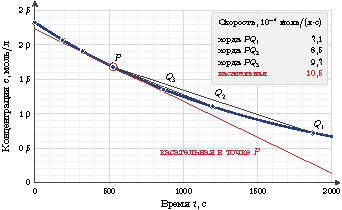
\includegraphics[width=12cm]{figs/what_is_reaction_rate/secants.pdf}
    \caption{Средние скорости разложения \ce{N2O5} на всё более коротких промежутках, начинающихся в точке $P$ ($t = \qty{526}{\ruS}$), приближаются к наклону касательной в этой точке. Наклоны хорд вычислены по данным табл.~\ref{tab:n2o5_decomposition}.}
    \label{fig:secants}
\end{figure}

Наклон касательной в точке представляет собой \term{мгновенную скорость}{instantaneous_rate}{мгновенная скорость}~--- предел, к которому стремится средняя скорость, если промежуток $\Delta t$ будет становиться всё меньше и меньше. В математике такой предел называют \emph{производной} и записывают как $\mathrm{d}c/\mathrm{d}t$. Буква d вместо $\Delta$ говорит о том, что изменения $c$ и $t$ бесконечно малы. Таким образом, мгновенная скорость по реагенту A равна
\begin{equation}
    \label{eq:instantaneous_rate}
    v(\mathrm{A}) = -\frac{\mathrm{d}c(\mathrm{A})}{\mathrm{d}t},
\end{equation}
а по продукту B будет равна $v(\mathrm{B}) = \mathrm{d}c(\mathrm{B})/\mathrm{d}t$ (без минуса).

На практике расчёт мгновенной скорости делается довольно просто. На графике проводят касательную к кривой в нужной точке, затем выбирают на ней две точки подальше друг от друга (на \emph{касательной}, а не на кривой) и делят разность концентраций на разность времён. Например, касательная на рис.~\ref{fig:secants} пересекает левую границу графика ($t = 0$) при $c \approx \qty{2,23}{\ruMole\per\ruL}$, а правую ($t = \qty{2000}{\ruS}$)~--- при $c \approx \qty{0,13}{\ruMole\per\ruL}$. Значит, в момент времени \qty{526}{\ruS}

\begin{equation*}
    v(\ce{N2O5}) \approx \frac{\num{2,23} - \num{0,13}}{2000 - 0} \approx \qty{1,05e-3}{\ruMole\per\ruL\ruS}.
\end{equation*}

Хорды, проведённые из $P$ к более \emph{ранним} точкам, дают значения скорости больше, чем в точке $P$: \qty{1,11e-3}{\ruMole\per\ruL\ruS} для промежутка \num{319}--\qty{526}{\ruS} и \qty{1,24e-3}{\ruMole\per\ruL\ruS} для промежутка \num{0}--\qty{526}{\ruS}. Таким образом, мгновенная скорость лежит между средними скоростями до и после рассматриваемой точки. При этом гораздо точнее её можно рассчитать по средней скорости на промежутке, который охватывает $P$ с обеих сторон. В данном случае для промежутка от 319 до \qty{867}{\ruS} она равна \qty{1,02e-3}{\ruMole\per\ruL\ruS}. Этим удобно пользоваться, когда касательную провести трудно (например, в задаче~\ref{prob:what_is_reaction_rate7}).

Особенно важной является мгновенная скорость в момент, когда реакция стартовала (при $t = 0$). Её называют \term{начальной скоростью}{initial_rate}{начальная скорость} реакции и обозначают $v_0$. В начале эксперимента состав реакционной смеси известен точно (мы же сами её приготовили), поэтому начальную скорость проще всего сопоставлять с концентрациями веществ. Так мы и будем поступать в следующих разделах. Для разложения \ce{N2O5} её можно найти по касательной к началу кинетической кривой на рис.~\ref{fig:kinetic_curves} (задача~\ref{prob:what_is_reaction_rate2}).

\subsection*{Скорость по веществу и скорость реакции}

Для реакций, в которых имеется несколько реагентов или продуктов, возникает вопрос: по какому веществу следить за реакцией? Для реакции~\eqref{ce:n2o5_decomposition} есть существенная разница в том, как это делать. Скорость роста концентрации \ce{N2O4} равна скорости падения концентрации \ce{N2O5}. Кислорода же за то же время образуется вдвое меньше, поскольку на каждые две разложившиеся молекулы \ce{N2O5} приходится одна образовавшаяся молекула \ce{O2}. Кислород при этом покидает раствор, так что говорить о его концентрации не имеет смысла, но скорость его образования в расчёте на литр раствора можно определить через количество вещества:

\begin{equation*}
    v(\ce{O2}) = \frac{1}{V}\,\frac{\mathrm{d}n(\ce{O2})}{\mathrm{d}t} = \frac{1}{2}\,v(\ce{N2O5}).
\end{equation*}

Скорости по разным веществам одной реакции могут различаться, но они всегда будут связаны между собой через коэффициенты в уравнении реакции. Как мы видели, когда \hyperref[sec:calculations_based_on_chemical_equations]{вели расчёты по уравнениям реакций}, количества прореагировавших и образовавшихся веществ пропорциональны их коэффициентам. Значит, и за любой промежуток времени количества всех участников меняются пропорционально коэффициентам, то есть величина $|\Delta n_i|/s_i$ для всех участников одна и та же. Поэтому, если разделить скорость по каждому веществу на его коэффициент, то для всех участников реакции получится одно и то же число. Его и называют \term{скоростью реакции}{reaction_rate}{скорость реакции}. Для реакции, в которой A~--- любой из реагентов, а B~--- любой из продуктов,

\begin{equation}
    \label{eq:reaction_rate}
    \boxed{v = -\frac{1}{s_{\mathrm{A}}}\,\frac{\mathrm{d}c(\mathrm{A})}{\mathrm{d}t} = \frac{1}{s_{\mathrm{B}}}\,\frac{\mathrm{d}c(\mathrm{B})}{\mathrm{d}t}},
\end{equation}

где $s_{\mathrm{A}}$ и $s_{\mathrm{B}}$~--- коэффициенты перед этими веществами в уравнении реакции\footnote{Формула~\eqref{eq:reaction_rate} верна, пока объём реакционной смеси не меняется, как, например, в растворе или в закрытом сосуде. В общем случае нам нужно представить эту формулу немного по-другому, где вместо изменения концентрации следует подставить изменение количества вещества, отнесённое к объёму: $v = \frac{1}{s_i V}\left|\frac{\mathrm{d}n_i}{\mathrm{d}t}\right|$. Так мы сделали с кислородом в объяснении выше.}. Для реакции разложения \ce{N2O5} по уравнению~\eqref{ce:n2o5_decomposition}

\begin{equation*}
    v = \frac{1}{2}\,v(\ce{N2O5}) = \frac{1}{2}\,v(\ce{N2O4}) = v(\ce{O2}).
\end{equation*}

Например, в момент времени, равный \qty{526}{\ruS}, \ce{N2O5} расходуется, а \ce{N2O4} образуется со скоростью \qty{1,05e-3}{\ruMole\per\ruL\ruS}, кислород образуется вдвое медленнее, со скоростью \qty{5,2e-4}{\ruMole\per\ruL\ruS}, и скорость реакции тоже равна \qty{5,2e-4}{\ruMole\per\ruL\ruS}.

При использовании скорости реакции есть нюанс, который заключается в том, что её значение зависит от того, \emph{как записано уравнение}. Если записать реакцию в виде \ce{N2O5 -> N2O4 + 1/2O2}, скорость реакции станет равной $v(\ce{N2O5})$, то есть вдвое больше, хотя в реальном мире ничего не изменилось. Но при этом скорости по веществам останутся прежними (потому что это измеряемые величины). Это аналогично тепловому эффекту \hyperref[term:thermochemical_equation]{термохимического уравнения}, который тоже удваивается при удвоении коэффициентов. Поэтому, говоря о скорости реакции, необходимо указывать и уравнение, к которому она относится.

\subsection*{Единицы скорости. Реакции на поверхности}

Скорость реакции обычно выражают в \unit{\ruMole\per\ruL\ruS}. Если процесс очень медленный, то можно использовать \unit{\ruMole\per\ruL\ruMin} или даже \unit{\ruMole\per\ruL\ruCh}. В системе СИ объём измеряют в кубических метрах, в этом случае $\qty{1}{\ruMole\per\ruL\ruS} = \qty{1000}{\ruMole\per\ruM\cubed\ruS}$.

Если реакция протекает в газовой фазе, то удобнее использовать не концентрации, а давления. Согласно уравнению состояния идеального газа~\eqref{eq:ideal_gas_law} $c = n/V = p/(RT)$, то есть при постоянной температуре концентрация газа пропорциональна его давлению (если мы рассматриваем смесь, то \emph{парциальному давлению}~--- той части общего давления, которая приходится на этот газ). Поэтому скорость газовой реакции можно выразить в единицах давления за единицу времени, например в \unit{\ruPa\per\ruS}, или перевести её при необходимости в \unit{\ruMole\per\ruM\cubed\ruS}, разделив на $RT$.

А что нам делать с реакциями, которые идут на поверхности (например, коррозия)? Назовём \term{фазой}{phase}{фаза} часть системы, одинаковую по составу и свойствам во всех своих точках и отделённую от остальных частей поверхностью раздела. Отдельной фазой будет являться раствор, кусок металла, газ над ними и т.~п. Если реакция протекает внутри одной фазы (например, в растворе или в газовой смеси), то её называют \term{гомогенной}{homogeneous_reaction}{гомогенная реакция}, а если на границе двух фаз (к примеру, металл в кислоте, горение угля, ржавление железа)~--- то \term{гетерогенной}{heterogeneous_reaction}{гетерогенная реакция}.

Гетерогенная реакция идёт только там, где фазы соприкасаются, поэтому её скорость относится не к объёму, а к площади поверхности раздела $A_{\text{пов}}$ и выражается в \unit{\ruMole\per\ruM\squared\ruS}:

\begin{equation}
    \label{eq:surface_reaction_rate}
    v = \frac{1}{s_i A_{\text{пов}}}\,\frac{|\Delta n_i|}{\Delta t}.
\end{equation}

Если мы разрежем металлическую пластинку на маленькие кусочки, то общая площадь поверхности станет больше и за секунду прореагирует больше металла, но в расчёте на квадратный метр скорость останется прежней.

Когда рассматривают реально протекающую коррозию (в инженерных расчётах), то вместо молей берут граммы, а вместо секунд~--- годы. К примеру, в городском воздухе сталь в результате коррозии теряет за год от 200 до \qty{400}{\ruG} металла с каждого квадратного метра поверхности, то есть слой толщиной \num{25}--\qty{50}{\ruUm}.

\subsection*{Как измерить скорость реакции}

Как это ни странно, не существует прибора, который показывал бы скорость реакции напрямую. На практике определение скорости заключается в измерении концентрации реагента или продукта (или величины, однозначно с ней связанной) в определённые моменты времени, а затем построении кинетической кривой и определении скорости по ней. При этом способы определения концентрации делятся на две большие группы.

\emph{Химические методы.} Из реакционной смеси через определённые промежутки времени отбирают небольшие объёмы проб и анализируют их, например титрованием или хроматографией. При этом во время измерения в пробе продолжается реакция, поэтому пробу тем или иным способом <<замораживают>>, например, резко охлаждают, сильно разбавляют или добавляют вещество, которое останавливает реакцию (например, связывают кислоту щёлочью). Это универсальный способ, впрочем, он даёт лишь отдельные точки.

\emph{Физические методы.} Также можно анализировать какое-либо свойство смеси, которое меняется в ходе реакции и связано с концентрацией веществ. Смесь при этом не трогают, а измерение чаще всего ведут непрерывно и записывают автоматически. Самые распространённые варианты таких методов приведены в табл.~\ref{tab:rate_measurement_methods}.

\begin{table}[htbp]
    \small
    \caption{Измеряемые показатели при определении скорости реакции.}
    \label{tab:rate_measurement_methods}
    \begin{tabularx}{\textwidth}{
        >{\hsize=0.85\hsize}Y
        >{\hsize=0.95\hsize}Y
        >{\hsize=1.2\hsize}Y
        }
        \hline
        \rowcolor{table_header}
        Что измеряют & Когда это возможно & Пример \\
        \hline
        Объём выделившегося газа & Выделяется газ, который легко собрать & \ce{2N2O5 -> 2N2O4 + O2 (^)} в растворе; \ce{Mg + 2HCl -> MgCl2 + H2 (^)} \\
        \hline
        Давление в закрытом сосуде & Реакция в газовой фазе, при которой меняется число молекул газа & \ce{2O3 -> 3O2}: из двух молекул газа получаются три \\
        \hline
        Массу реакционной смеси & Газ уходит из открытого сосуда & \ce{CaCO3 + 2HCl -> CaCl2 + H2O + CO2 (^)} \\
        \hline
        Окраску (поглощение света) & Хотя бы один из участников окрашен & Раствор перманганата калия обесцвечивается щавелевой кислотой \\
        \hline
        Электропроводность раствора & Меняется число ионов в растворе & \ce{(CH3)3CCl + H2O -> (CH3)3COH + HCl}: в растворе появляются ионы \ce{H+} и \ce{Cl-} \\
        \hline
        Угол поворота плоскости поляризации света & Участвуют оптически активные вещества & Гидролиз сахарозы \\
        \hline
    \end{tabularx}
\end{table}

Например, чем больше в растворе окрашенного вещества, тем сильнее он поглощает свет. Это можно измерить при помощи фотоколориметра, который показывает, какая доля исходного света прошла через раствор (не поглотилась). Также растворы некоторых веществ (например, сахаров) поворачивают плоскость поляризации проходящего через них света, и угол поворота пропорционален концентрации. Угол поворота измеряют при помощи прибора, называющегося поляриметром. Именно так впервые в истории удалось измерить скорость химической реакции (немецкий физик Людвиг Вильгельми в 1850~году измерил скорость гидролиза сахарозы в присутствии кислоты).

Данные, приведённые в табл.~\ref{tab:n2o5_decomposition}, получены расчётным путём по объёму выделившегося газа. Эйринг и Даниэлс собирали выделявшийся кислород в газовую бюретку и измеряли его объём, а концентрации \ce{N2O5} вычислены из этого объёма по уравнению реакции\footnote{Колба вместимостью \qty{5}{\ruMl} с раствором находилась в термостате, где температура колебалась не больше чем на \qty{0,01}{\degreeCelsius}. Колбу встряхивали 360~раз в минуту. Это нужно было для того, чтобы кислород не оставался в растворе. Выделяющийся газ проходил через стекловату, смоченную концентрированной серной кислотой, которая поглощала диоксид азота, тоже присутствовавший в газовой смеси.}. Упрощённая схема этого эксперимента и его результаты показаны на рис.~\ref{fig:gas_syringe}.

\begin{figure}[htbp]
    \centering
    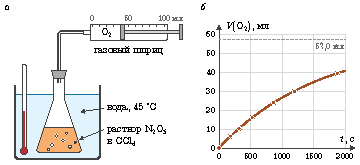
\includegraphics[width=12cm]{figs/what_is_reaction_rate/gas_syringe.pdf}
    \caption{Эксперимент по измерению скорости разложения \ce{N2O5} через объём выделившегося кислорода: \emph{а}~--- упрощённая схема опыта: колба с раствором стоит в термостате при \qty{45}{\degreeCelsius}, кислород собирается в газовый шприц; \emph{б}~--- объём выделившегося кислорода для \qty{2,00}{\ruMl} раствора из табл.~\ref{tab:n2o5_decomposition} (в пересчёте на \qty{25}{\degreeCelsius} и \qty{101,3}{\ruKPa}). Пунктир~--- объём после полного разложения \ce{N2O5}.}
    \label{fig:gas_syringe}
\end{figure}

\begin{example}{}{what_is_reaction_rate2}
    \begin{condition}
        В колбу налили \qty{2,00}{\ruMl} раствора \ce{N2O5} в \ce{CCl4} из табл.~\ref{tab:n2o5_decomposition}. За первые \qty{184}{\ruS} в шприце собралось \qty{6,25}{\ruMl} кислорода (объём приведён к \qty{25}{\degreeCelsius} и давлению \qty{101,3}{\ruKPa}). Какова концентрация \ce{N2O5} в этот момент? Какой объём кислорода соберётся, когда весь \ce{N2O5} разложится?
    \end{condition}

    \medskip

    \textit{Решение.} Количество кислорода найдём из уравнения состояния идеального газа~\eqref{eq:ideal_gas_law}:

    \begin{equation*}
        n(\ce{O2}) = \frac{pV}{RT} = \frac{\num{101300} \cdot \num{6,25e-6}}{\num{8,314} \cdot 298} = \qty{2,56e-4}{\ruMole}.
    \end{equation*}

    По уравнению~\eqref{ce:n2o5_decomposition} две молекулы \ce{N2O5} приводят к образованию одной молекулы кислорода, поэтому к этому моменту разложилось $2n(\ce{O2}) = \qty{5,12e-4}{\ruMole}$ \ce{N2O5}, и его концентрация уменьшилась на

    \begin{equation*}
        \Delta c = \frac{\qty{5,12e-4}{\ruMole}}{\qty{2,00e-3}{\ruL}} = \qty{0,256}{\ruMole\per\ruL}.
    \end{equation*}

    К моменту времени \qty{184}{\ruS} концентрация \ce{N2O5} стала равна $\num{2,33} - \num{0,256} \approx \qty{2,07}{\ruMole\per\ruL}$ (это значение и стоит в табл.~\ref{tab:n2o5_decomposition})\footnote{Вместе с кислородом из колбы уходят ещё и пары растворителя. Но мы для простоты считаем газ в шприце чистым кислородом.}.

    К моменту окончания реакции кислорода выделится вдвое меньше, чем изначально было \ce{N2O5}:
    \begin{equation*}
        n(\ce{O2}) = \frac{1}{2} \cdot \qty{2,33}{\ruMole\per\ruL} \cdot \qty{2,00e-3}{\ruL} = \qty{2,33e-3}{\ruMole},
    \end{equation*}
    то есть
    \begin{equation*}
        V = \frac{nRT}{p} = \frac{\num{2,33e-3} \cdot \num{8,314} \cdot 298}{\num{101300}} = \qty{5,70e-5}{\ruM\cubed} = \qty{57,0}{\ruMl}.
    \end{equation*}

    Этот объём показан на рис.~\ref{fig:gas_syringe} пунктиром.
\end{example}

Однако для очень быстрых реакций такие способы измерения скорости непригодны, потому что реакция закончится раньше, чем мы успеем смешать растворы. В этом случае реакцию инициируют импульсом света или резким нагревом, а затем следят за ней оптическими методами. За исследования таких быстропротекающих реакций Манфред Эйген, Рональд Норриш и Джордж Портер получили Нобелевскую премию по химии 1967~года. Позже с помощью лазерных импульсов длительностью в десятки фемтосекунд (фемтосекунда~--- это \qty{e-15}{\ruS}) удалось даже наблюдать момент, когда рвутся и образуются химические связи. Эта работа Ахмеда Зевейла была удостоена Нобелевской премии 1999~года.

\subsection*{Некоторые подводные камни}

Вам нужно чётко понимать, какую информацию несёт в себе скорость химической реакции, а какую не несёт.

Во-первых, скорость реакции ничего не говорит о том, чем закончится реакция. Для описания того, \emph{сколько} в итоге получилось продукта, используются \hyperref[term:yield]{выход реакции} и полнота превращения. Например, быстро протекающая реакция может дать низкий выход продукта, если параллельно с ней будут идти побочные реакции. Напротив, медленная реакция рано или поздно может пройти до конца. В этой главе мы пока будем считать, что реакции идут только в одну сторону, до полного расходования одного из реагентов.

Во-вторых, скорость реакции не определяется энергией Гиббса. Знак $\Delta G$ говорит, \emph{может ли} реакция идти, но не говорит, \emph{как быстро} она будет протекать. Реакция может быть термодинамически очень выгодной, но при этом идти невероятно медленно (например, превращение алмаза в графит из задачи~\ref{prob:gibbs_energy7} или взаимодействие водорода с кислородом при комнатной температуре). И наоборот, реакция с небольшим энергетическим выигрышем может идти мгновенно (задача~\ref{prob:what_is_reaction_rate5}). Термодинамика указывает только, в какую сторону будет идти реакция, а кинетика~--- как быстро и каким путём.

\begin{termlist}
    \hyperref[term:chemical_kinetics]{Химическая кинетика},
    \hyperref[term:kinetic_curve]{кинетическая кривая},
    \hyperref[term:average_rate]{средняя скорость},
    \hyperref[term:rate_by_substance]{скорость по веществу},
    \hyperref[term:instantaneous_rate]{мгновенная скорость},
    \hyperref[term:initial_rate]{начальная скорость},
    \hyperref[term:reaction_rate]{скорость реакции},
    \hyperref[term:phase]{фаза},
    \hyperref[term:homogeneous_reaction]{гомогенная реакция},
    \hyperref[term:heterogeneous_reaction]{гетерогенная реакция}.
\end{termlist}

\begin{problem}{}{what_is_reaction_rate1}
    По данным табл.~\ref{tab:n2o5_decomposition} вычислите средние скорости разложения \ce{N2O5} на каждом из шести промежутков между соседними измерениями. Как меняется скорость со временем? Сколько \ce{N2O5} разложилось бы за первые \qty{184}{\ruS}, если бы реакция в течение всего времени шла со средней скоростью за всё время наблюдения, найденной в примере~\ref{ex:what_is_reaction_rate1}? Проведите сравнение с тем, что было на самом деле.
    \begin{sol}{\ref{prob:what_is_reaction_rate1}}
        По формуле~\eqref{eq:average_rate} получаем:

        \begin{center}
            \small
            \begin{tabular}{cccc}
                \hline
                \rowcolor{table_header}
                Промежуток, с & $\Delta c$, \unit{\ruMole\per\ruL} & $\Delta t$, с & $\overline{v}$, \unit{\ruMole\per\ruL\ruS} \\
                \hline
                0--184 & \num{0,26} & 184 & \num{1,41e-3} \\
                184--319 & \num{0,16} & 135 & \num{1,19e-3} \\
                319--526 & \num{0,23} & 207 & \num{1,11e-3} \\
                526--867 & \num{0,33} & 341 & \num{9,7e-4} \\
                867--1198 & \num{0,24} & 331 & \num{7,3e-4} \\
                1198--1877 & \num{0,39} & 679 & \num{5,7e-4} \\
                \hline
            \end{tabular}
        \end{center}

        Скорость реакции монотонно уменьшается. К концу опыта она упала почти в два с половиной раза. Если бы реакция всё время шла со средней скоростью \qty{8,58e-4}{\ruMole\per\ruL\ruS}, за первые \qty{184}{\ruS} разложилось бы $\num{8,58e-4} \cdot 184 \approx \qty{0,16}{\ruMole\per\ruL}$ \ce{N2O5}, а на самом деле разложилось \qty{0,26}{\ruMole\per\ruL}, в \num{1,6}~раза больше.
    \end{sol}
\end{problem}

\begin{problem}{}{what_is_reaction_rate2}
    На рис.~\ref{fig:kinetic_curves} проведены касательные к кинетическим кривым в начальный момент времени и в момент $t = \qty{1700}{\ruS}$.
    \begin{enumerate}[label=\arabic*)]
        \item По касательным найдите начальную скорость разложения \ce{N2O5} и скорость в момент $t = \qty{1700}{\ruS}$.
        \item Чему равны в эти моменты скорость образования \ce{N2O4}, скорость образования кислорода (в расчёте на литр раствора) и скорость реакции~\eqref{ce:n2o5_decomposition}?
        \item Во сколько раз уменьшилась скорость разложения \ce{N2O5} за \qty{1700}{\ruS}? Во сколько раз за то же время уменьшилась концентрация \ce{N2O5} (её значение в момент $t = \qty{1700}{\ruS}$ найдите по графику)?
    \end{enumerate}
    \begin{sol}{\ref{prob:what_is_reaction_rate2}}
        1)~Начальная касательная проходит через точки (0;~\num{2,33}) и (500;~\num{1,60}), поэтому

        \begin{equation*}
            v_0(\ce{N2O5}) = \frac{\num{2,33} - \num{1,60}}{500} = \qty{1,46e-3}{\ruMole\per\ruL\ruS}.
        \end{equation*}

        Касательная в момент $t = \qty{1700}{\ruS}$ проходит через точки (1200;~\num{1,06}) и (2200;~\num{0,55}), и

        \begin{equation*}
            v(\ce{N2O5}) = \frac{\num{1,06} - \num{0,55}}{1000} = \qty{5,1e-4}{\ruMole\per\ruL\ruS}.
        \end{equation*}

        Ваши значения могут немного отличаться~--- это не страшно: всё зависит от того, насколько точно вы считываете координаты с графика.

        2)~Касательные к кривой \ce{N2O4} зеркальны касательным к кривой \ce{N2O5}, поэтому \ce{N2O4} образуется с той же скоростью \num{1,46e-3} и \qty{5,1e-4}{\ruMole\per\ruL\ruS}. Кислорода по уравнению~\eqref{ce:n2o5_decomposition} образуется вдвое меньше, около \num{7,3e-4} и \qty{2,5e-4}{\ruMole\per\ruL\ruS}. Скорость реакции по формуле~\eqref{eq:reaction_rate} равна $v = \frac{1}{2}v(\ce{N2O5})$, то есть тоже \num{7,3e-4} и \qty{2,5e-4}{\ruMole\per\ruL\ruS}.

        3)~Скорость уменьшилась в $\num{1,46e-3}/\num{5,1e-4} \approx \num{2,9}$~раза. Концентрация \ce{N2O5} в момент $t = \qty{1700}{\ruS}$ по графику около \qty{0,81}{\ruMole\per\ruL}, то есть она уменьшилась в $\num{2,33}/\num{0,81} \approx \num{2,9}$~раза~--- так же, как и скорость. Это логично, поскольку скорость этой реакции пропорциональна концентрации \ce{N2O5}. Подробнее об этом~--- в следующем разделе.
    \end{sol}
\end{problem}

\begin{problem}{}{what_is_reaction_rate3}
    Реакцию пероксида водорода с иодидом калия в кислой среде
    \reaction*{H2O2 + 2KI + H2SO4 -> I2 + K2SO4 + 2H2O}
    одной из первых изучили количественно (ещё в 1860-х годах). В некоторый момент времени иод образуется со скоростью \qty{2,0e-5}{\ruMole\per\ruL\ruS}.
    \begin{enumerate}[label=\arabic*)]
        \item С какой скоростью в этот момент расходуются пероксид водорода, иодид калия и серная кислота? Чему равна скорость реакции?
        \item Выразите скорость расходования иодида калия в \unit{\ruMole\per\ruL\ruMin} и в \unit{\ruMole\per\ruM\cubed\ruS}.
        \item Как изменятся найденные величины, если записать уравнение с коэффициентами, вдвое меньшими?
    \end{enumerate}
    \begin{sol}{\ref{prob:what_is_reaction_rate3}}
        1)~По формуле~\eqref{eq:reaction_rate} скорость реакции равна скорости образования иода, делённой на его коэффициент:
        \begin{equation*}
            v = \frac{v(\ce{I2})}{1} = \qty{2,0e-5}{\ruMole\per\ruL\ruS}.
        \end{equation*}

        Отсюда
        \begin{equation*}
            v(\ce{H2O2}) = v(\ce{H2SO4}) = v = \qty{2,0e-5}{\ruMole\per\ruL\ruS},
        \end{equation*}
        \begin{equation*}
            v(\ce{KI}) = 2v = \qty{4,0e-5}{\ruMole\per\ruL\ruS}.
        \end{equation*}

        2)~Минута в 60 раз длиннее секунды, а кубический метр в 1000 раз больше литра:
        \begin{equation*}
            \qty{4,0e-5}{\ruMole\per\ruL\ruS} \cdot \qty{60}{\ruS\per\ruMin} = \qty{2,4e-3}{\ruMole\per\ruL\ruMin},
        \end{equation*}
        \begin{equation*}
            \qty{4,0e-5}{\ruMole\per\ruL\ruS} \cdot \qty{1000}{\ruL\per\ruM\cubed} = \qty{4,0e-2}{\ruMole\per\ruM\cubed\ruS}.
        \end{equation*}

        3)~Скорости по веществам~--- это измеряемые величины, поэтому от записи уравнения они не зависят. А вот скорость реакции вырастет вдвое:
        \begin{equation*}
            v = \frac{v(\ce{I2})}{1/2} = \qty{4,0e-5}{\ruMole\per\ruL\ruS}.
        \end{equation*}
    \end{sol}
\end{problem}

\begin{problem}{}{what_is_reaction_rate4}
    Каким способом вы бы предпочли следить за ходом каждой из указанных реакций? Объясните свой выбор.
    \begin{enumerate}[label=\arabic*)]
        \item Кусочки мрамора растворяются в соляной кислоте: \ce{CaCO3 + 2HCl -> CaCl2 + H2O + CO2 (^)}.
        \item Цинковая пластинка опущена в раствор сульфата меди (II): \ce{Zn + CuSO4 -> ZnSO4 + Cu}.
        \item При \qty{500}{\degreeCelsius} циклопропан превращается в пропен \ce{CH2=CH-CH3}; оба вещества~--- бесцветные газы.
        \item Озон разлагается в закрытом сосуде: \ce{2O3 -> 3O2}.
        \item Этилацетат гидролизуется раствором гидроксида натрия: \ce{CH3COOC2H5 + NaOH -> CH3COONa + C2H5OH}.
    \end{enumerate}
    \begin{sol}{\ref{prob:what_is_reaction_rate4}}
        1)~Углекислый газ уходит из открытой колбы, поэтому удобно поставить колбу на весы и следить за уменьшением массы (горлышко закрывают ватой, чтобы вместе с газом не вылетали брызги кислоты). Можно также собирать газ в шприц.

        2)~Раствор сульфата меди (II) голубой, а сульфат цинка бесцветен, поэтому окраска бледнеет по мере протекания реакции, и за ней можно следить фотоколориметром.

        3)~Здесь из одной молекулы газа получается одна молекула газа, поэтому давление в закрытом сосуде не меняется, при этом оба газа бесцветны. Что ж, остаётся только отбирать пробы и анализировать их состав.

        4)~Из двух молекул газа получаются три, поэтому давление в закрытом сосуде растёт (после окончания реакции оно вырастет в полтора раза). Также можно использовать способность озона поглощать ультрафиолетовое излучение.

        5)~Щёлочь расходуется, поэтому можно отбирать пробы, <<замораживать>> их избытком кислоты известной концентрации, а затем оттитровывать остаток кислоты. Также можно следить за электропроводностью, используя тот факт, что гидроксид-ионы проводят ток гораздо лучше ацетат-ионов, которые их заменяют, из-за чего электропроводность раствора будет падать по мере протекания реакции.
    \end{sol}
\end{problem}

\begin{problem}{}{what_is_reaction_rate5}
    Профессор Недоумелкин сравнивает реакции: образование воды из водорода и кислорода ($\Delta G^{\circ} = \qty{-237}{\ruKJ}$ на моль воды) и нейтрализацию соляной кислоты гидроксидом натрия ($\Delta G^{\circ} \approx \qty{-80}{\ruKJ}$ на моль воды). <<Первая реакция втрое выгоднее, значит, она и идёт втрое быстрее>>,~--- заключает он. Что вы ему ответите?
    \begin{sol}{\ref{prob:what_is_reaction_rate5}}
        Энергия Гиббса отвечает на вопрос, может ли реакция идти, но ничего не говорит о её скорости. На деле смесь водорода с кислородом при комнатной температуре может годами храниться без заметных изменений, пока её не подожгут, а нейтрализация в растворе проходит мгновенно. Ионы \ce{H+} и \ce{OH-} соединяются практически при каждой встрече~--- это одна из самых быстрых реакций в растворе. На практике её скорость ограничивает скорость перемешивания растворов.

        Можно рассуждать и по-другому. Если поджечь смесь водорода с кислородом, то скорость реакции вырастет на много порядков, хотя $\Delta G$ останется прежним. Значит, скорость определяется чем-то другим. Чем именно, мы объясним в следующих разделах.
    \end{sol}
\end{problem}

\begin{problem}{}{what_is_reaction_rate6}
    $\bigstar$ Ленту магния массой \qty{0,048}{\ruG} опустили в \qty{50,0}{\ruMl} соляной кислоты с концентрацией \qty{1,00}{\ruMole\per\ruL}, а выделяющийся водород собирали в газовый шприц. За первые \qty{30}{\ruS} набралось \qty{24,0}{\ruMl} газа при \qty{20}{\degreeCelsius} и \qty{101,3}{\ruKPa}.
    \begin{enumerate}[label=\arabic*)]
        \item Какое количество водорода выделилось и какая доля магния успела прореагировать?
        \item Найдите среднюю скорость расходования \ce{HCl} и среднюю скорость реакции за эти \qty{30}{\ruS} в \unit{\ruMole\per\ruL\ruS}. Как при этом изменилась концентрация кислоты?
        \item Реакция идёт на поверхности металла, площадь которой в начале опыта около \qty{3,0}{\ruCm\squared}. Найдите среднюю скорость реакции в \unit{\ruMole\per\ruM\squared\ruS}.
        \item Во сколько раз магний растворяется в кислоте быстрее, чем ржавеет сталь в городском воздухе (\num{200}--\qty{400}{\ruG} железа с квадратного метра в год)?
    \end{enumerate}
    \begin{sol}{\ref{prob:what_is_reaction_rate6}}
        1)~Из уравнения состояния идеального газа
        \begin{equation*}
            n(\ce{H2}) = \frac{pV}{RT} = \frac{\num{101300} \cdot \num{24,0e-6}}{\num{8,314} \cdot 293} = \num{9,98e-4} \approx \qty{1,00e-3}{\ruMole}.
        \end{equation*}

        Магния было $\num{0,048}/\num{24,31} = \qty{1,97e-3}{\ruMole}$. По уравнению \ce{Mg + 2HCl -> MgCl2 + H2 (^)} на каждый моль водорода расходуется моль магния, значит, прореагировала примерно половина магния.

        2)~Кислоты израсходовано вдвое больше, чем выделилось водорода: $\Delta n(\ce{HCl}) = \qty{2,00e-3}{\ruMole}$, поэтому
        \begin{equation*}
            \Delta c(\ce{HCl}) = \frac{\qty{2,00e-3}{\ruMole}}{\qty{0,0500}{\ruL}} = \qty{0,0400}{\ruMole\per\ruL},
        \end{equation*}
        а средняя скорость расходования \ce{HCl} за \qty{30}{\ruS}
        \begin{equation*}
            \overline{v}(\ce{HCl}) = \frac{\qty{0,0400}{\ruMole\per\ruL}}{\qty{30}{\ruS}} = \qty{1,33e-3}{\ruMole\per\ruL\ruS}.
        \end{equation*}

        Скорость реакции по формуле~\eqref{eq:reaction_rate} вдвое меньше: \qty{6,7e-4}{\ruMole\per\ruL\ruS}. Концентрация кислоты уменьшилась всего с \num{1,00} до \qty{0,96}{\ruMole\per\ruL}, потому что кислота взята в большом избытке.

        3)~По формуле~\eqref{eq:surface_reaction_rate}
        \begin{equation*}
            v = \frac{\num{1,00e-3}}{\num{3,0e-4} \cdot 30} \approx \qty{0,11}{\ruMole\per\ruM\squared\ruS}.
        \end{equation*}

        4)~Сталь теряет \num{200}--\qty{400}{\ruG}, то есть \num{3,6}--\qty{7,2}{\ruMole} железа с квадратного метра за год, а в году \qty{3,16e7}{\ruS}. Это \num{1,1e-7}--\qty{2,3e-7}{\ruMole\per\ruM\squared\ruS}. Отношение скоростей
        \begin{equation*}
            \frac{\num{0,11}}{\num{2,3e-7}} \approx \num{5e5} \quad\text{и}\quad \frac{\num{0,11}}{\num{1,1e-7}} \approx \num{1e6},
        \end{equation*}
        то есть магний в кислоте растворяется в полмиллиона~--- миллион раз быстрее.
    \end{sol}
\end{problem}

\begin{problem}{}{what_is_reaction_rate7}
    $\bigstar$ Если трудно провести касательную к кинетической кривой, мгновенную скорость оценивают через среднюю скорость на коротком промежутке (точка при этом должна лежать на его середине).
    \begin{enumerate}[label=\arabic*)]
        \item Используя результаты задачи~\ref{prob:what_is_reaction_rate1}, постройте график зависимости скорости разложения \ce{N2O5} от времени, откладывая каждую среднюю скорость в середине своего промежутка.
        \item Для каждого промежутка найдите среднюю концентрацию \ce{N2O5} (полусумму значений на его концах) и постройте график зависимости скорости от концентрации. Что вы замечаете?
        \item С какой скоростью разлагался бы \ce{N2O5} в растворе с концентрацией \qty{1,00}{\ruMole\per\ruL} при той же температуре?
    \end{enumerate}
    \begin{sol}{\ref{prob:what_is_reaction_rate7}}
        1)~Середины промежутков приходятся на 92, 252, 423, 697, 1033 и \qty{1538}{\ruS}, а скорости (в единицах \qty{e-4}{\ruMole\per\ruL\ruS}) равны \num{14,1}; \num{11,9}; \num{11,1}; \num{9,7}; \num{7,3} и \num{5,7}. Точки ложатся на плавную убывающую кривую, похожую по форме на саму кинетическую кривую \ce{N2O5}.

        2)~Средние концентрации равны \num{2,20}; \num{1,99}; \num{1,80}; \num{1,52}; \num{1,23} и \qty{0,92}{\ruMole\per\ruL}. На графике <<скорость~--- концентрация>> точки ложатся на прямую, проходящую через начало координат: отношение скорости к концентрации почти одно и то же, от \num{5,9e-4} до \qty{6,4e-4}{\ruS\tothe{-1}}, в среднем \qty{6,2e-4}{\ruS\tothe{-1}}. Значит, скорость разложения \ce{N2O5} пропорциональна его концентрации. Именно поэтому в задаче~\ref{prob:what_is_reaction_rate2} скорость и концентрация уменьшились в одно и то же число раз.

        3)~Скорость пропорциональна концентрации, поэтому
        \begin{equation*}
            v = \qty{6,2e-4}{\ruS\tothe{-1}} \cdot \qty{1,00}{\ruMole\per\ruL} = \qty{6,2e-4}{\ruMole\per\ruL\ruS}.
        \end{equation*}

        Такие зависимости скорости от концентрации мы будем изучать в следующем разделе. Настоящий опыт дал бы чуть меньшее значение: Эйринг и Даниэлс заметили, что в растворах с меньшей начальной концентрацией отношение скорости к концентрации немного меньше. В опыте, начатом с \qty{1,40}{\ruMole\per\ruL}, оно было в среднем \qty{6,0e-4}{\ruS\tothe{-1}}.
    \end{sol}
\end{problem}

\clearpage